\documentclass{article}
\usepackage{tikz}
\usepackage{calc}
\begin{document}

\begin{figure}\centering
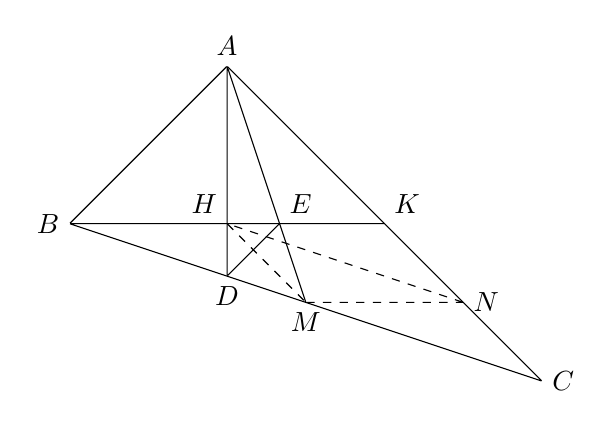
\begin{tikzpicture}
[
enode/.style={circle, minimum size=0mm, inner sep=0}
]
\node[enode, label={90:$A$}] (A) at  ( 0,  2) {};
\node[enode, label={180:$B$}] (B) at (-2,  0) {};
\node[enode, label={ 80:$K$}] (K) at ( 2,  0) {};
\node[enode, label={140:$H$}] (H) at ( 0,  0) {};
\node[enode, label={-90:$D$}] (D) at ( 0, -0.66666) {};
\node[enode, label={ 50:$E$}] (E) at ( 0.6666667, 0) {};
\node[enode, label={  0:$C$}] (C) at ( 4, -2) {};
\node[enode, label={-90:$M$}] (M) at ( 1, -1.0) {};
\node[enode, label={  0:$N$}] (N) at ( 3, -1.0) {};

\draw (B) to (C) to (A) to (B) to (K);
\draw (M) to (A) to (D) to (E);
\draw[dashed] (M) to (N) to (H) to (M);
\end{tikzpicture}
\end{figure}

\end{document}
